\documentclass{article}

\usepackage{amsthm}
\usepackage{amsfonts}
\usepackage{amsmath}
\usepackage{amssymb}
\usepackage{array}
\usepackage{enumitem}
\usepackage{fullpage}
\usepackage[usenames]{color}
\usepackage{hyperref}
  \hypersetup{
    colorlinks = true,
    urlcolor = blue,       % color of external links using \href
    linkcolor= blue,       % color of internal links 
    citecolor= blue,       % color of links to bibliography
    filecolor= blue,        % color of file links
    }
    
\usepackage{listings}
\usepackage{parskip}
\usepackage{qtree}
\usepackage{tikz-qtree}

\definecolor{dkgreen}{rgb}{0,0.6,0}
\definecolor{gray}{rgb}{0.5,0.5,0.5}
\definecolor{mauve}{rgb}{0.58,0,0.82}

\lstset{frame=tb,
  language=haskell,
  aboveskip=3mm,
  belowskip=3mm,
  showstringspaces=false,
  columns=flexible,
  basicstyle={\small\ttfamily},
  numbers=none,
  numberstyle=\tiny\color{gray},
  keywordstyle=\color{blue},
  commentstyle=\color{dkgreen},
  stringstyle=\color{mauve},
  breaklines=true,
  breakatwhitespace=true,
  tabsize=3
}

\theoremstyle{theorem} 
   \newtheorem{theorem}{Theorem}[section]
   \newtheorem{corollary}[theorem]{Corollary}
   \newtheorem{lemma}[theorem]{Lemma}
   \newtheorem{proposition}[theorem]{Proposition}
\theoremstyle{definition}
   \newtheorem{definition}[theorem]{Definition}
   \newtheorem{example}[theorem]{Example}
\theoremstyle{remark}    
  \newtheorem{remark}[theorem]{Remark}


\title{CPSC-354 Report}
\author{Eleas Vrahnos  \\ Chapman University}

\date{\today}

\begin{document}

\maketitle

\begin{abstract}
\noindent Every computer needs their own set of instructions and syntax in order to communicate with users and other computers. Programming languages are these sets of instructions that instruct a computer how to operate. The most popular programming languages used by developers and programmers today include Python, JavaScript, and C++. Even though these languages are different in many ways, they all originated from their own basic building blocks. These building blocks make each programming language unique in their use and functionality. For example, the difference between interpreted vs. compiled languages can lead to tradeoffs between syntax simplicity and performance issues. Each programming language has their own advantages and disadvantages, and the way they are structured determines what strengths and weaknesses it will have. This report aims to highlight what these building blocks are and how they can be used to build a fully functional programming language. This will be done through explorations of various concepts such as syntax trees, abstract reduction systems, and recursion applications. A final software project will also be showcased at the end, investigating how the Ruby programming language compares to other languages.
\end{abstract}

\tableofcontents

\section{Introduction}\label{intro}

This report is written by Eleas Vrahnos, a third-year undergraduate at Chapman University at the time of this report's completion. It details all assignments and progress made in the Programming Languages course, CPSC 354. It includes weekly homework assigments and a final project that demonstrate understanding and application in various class topics covered that week. These exercises are coded through concepts gained from Haskell, BNF, and lambda calculus. These are used to help make creating an example programming language interpreter as simple and powerful as possible.
\newpage

\section{Homework}\label{homework}

This section will contain my solutions to the weekly homework assignments. 

\subsection{Week 1}

The following is a Python implementation of the Euclidean algorithm, a method for computing the greatest common divisor between two integers. A sample input \texttt{gcd(9, 33)} is tested step by step below.

\begin{lstlisting}[language=Python]
def gcd(a,b):
    while a != b:
        if a > b: a = a-b
        else: b = b-a
    return a
\end{lstlisting}
\begin{enumerate}[noitemsep]
  \item \texttt{gcd(9, 33)}
  \begin{itemize}
      \item The function is called, assigning 9 to variable \texttt{a} and 33 to variable \texttt{b}.
  \end{itemize} 
  \item \texttt{while a != b:}
  \begin{itemize}
      \item The while loop condition returns True, so the loop starts.
  \end{itemize}
  \item \texttt{else:}
  \begin{itemize}
      \item \texttt{a > b} (9 $>$ 33) returns False, so the else block executes.
  \end{itemize}
  \item \texttt{b = b-a}
  \begin{itemize}
      \item \texttt{b} is now assigned to $33 - 9$, which is $24$.
  \end{itemize}
  \item \texttt{while a != b:}
  \begin{itemize}
      \item The while loop condition returns True, so the loop starts.
  \end{itemize}
  \item \texttt{else:}
  \begin{itemize}
      \item \texttt{a > b} (9 $>$ 24) returns False, so the else block executes.
  \end{itemize}
  \item \texttt{b = b-a}
  \begin{itemize}
      \item \texttt{b} is now assigned to $24 - 9$, which is $15$.
  \end{itemize}
  \item \texttt{while a != b:}
  \begin{itemize}
      \item The while loop condition returns True, so the loop starts.
  \end{itemize}
  \item \texttt{else:}
  \begin{itemize}
      \item \texttt{a > b} (9 $>$ 15) returns False, so the else block executes.
  \end{itemize}
  \item \texttt{b = b-a}
  \begin{itemize}
      \item \texttt{b} is now assigned to $15 - 9$, which is $6$.
  \end{itemize}
  \item \texttt{while a != b:}
  \begin{itemize}
      \item The while loop condition returns True, so the loop starts.
  \end{itemize}
  \item \texttt{if a > b:}
  \begin{itemize}
      \item \texttt{a > b} (9 $>$ 6) returns True, so the first block executes.
  \end{itemize}
  \item \texttt{a = a-b}
  \begin{itemize}
      \item \texttt{a} is now assigned to $9 - 6$, which is $3$.
  \end{itemize}
  \item \texttt{while a != b:}
  \begin{itemize}
      \item The while loop condition returns True, so the loop starts.
  \end{itemize}
  \item \texttt{else:}
  \begin{itemize}
      \item \texttt{a > b} (3 $>$ 6) returns False, so the else block executes.
  \end{itemize}
  \item \texttt{b = b-a}
  \begin{itemize}
      \item \texttt{b} is now assigned to $6 - 3$, which is $3$.
  \end{itemize}
  \item \texttt{while a != b:}
  \begin{itemize}
      \item The while loop condition returns False (\texttt{3 == 3}), so the loop ends.
  \end{itemize}
  \item \texttt{return a}
  \begin{itemize}
      \item \texttt{a} is returned from the function, giving the correct greatest common divisor of \textbf{3}.
  \end{itemize}
\end{enumerate}

\subsection{Week 2}

The following are implementations of various functions in Haskell and corresponding examples. For the execution sequences, equational reasoning is shown in the comments by line number of the implementation.

% select_evens function
\noindent \texttt{select\_evens}, lists the even-indexed elements of a given list:
\begin{lstlisting}[language=Haskell]
-- Implementation
select_evens [] = [] -- in the case of a list with even number elements
select_evens (x:[]) = [] -- in the case of a list with odd number elements
select_evens (x:y:xs) = y : select_evens (xs)

-- Execution Sequence with example ["a","b","c","d","e"]
select_evens ["a","b","c","d","e"]
    = "b" : (select_evens["c","d","e"]) -- line 3
    = "b" : ("d" : (select_evens["e"])) -- line 3
    = "b" : ("d" : ([])) -- line 2
    = ["b","d"] -- line 1
\end{lstlisting} 

% select_odds function
\noindent \texttt{select\_odds}, lists the odd-indexed elements of a given list:
\begin{lstlisting}[language=Haskell]
-- Implementation
select_odds [] = [] -- in the case of a list with even number elements
select_odds (x:[]) = [x] -- in the case of a list with odd number elements
select_odds (x:y:xs) = x : select_odds (xs)

-- Execution Sequence with example ["a","b","c","d","e"]
select_odds ["a","b","c","d","e"]
    = "a" : (select_odds["c","d","e"]) -- line 3
    = "a" : ("c" : (select_odds["e"])) -- line 3
    = "a" : ("c" : ("e")) -- line 2
    = ["a","c","e"] -- syntax of lists
\end{lstlisting}

% member function
\noindent \texttt{member}, determines whether an element is part of a given list:
\begin{lstlisting}[language=Haskell]
-- Implementation
member a [] = False
member a (x:xs)
    | a==x = True
    | otherwise = member a (xs)

-- Execution Sequence with example 2 [5,2,6]
member 2 [5,2,6]
    = member 2 [2,6] -- lines 2 -> 4
    = True -- lines 2 -> 3
\end{lstlisting}

\newpage

% append function
\noindent \texttt{append}, appends a list to another list:
\begin{lstlisting}[language=Haskell]
-- Implementation
append [] ys = ys
append (x:xs) ys = x : append xs ys

-- Execution Sequence with example [1,2] [3,4,5]
append [1,2] [3,4,5]
    = 1 : (append [2] [3,4,5]) -- line 2
    = 1 : (2 : (append [] [3,4,5])) -- line 2
    = 1 : (2 : ([3,4,5])) -- line 1
    = [1,2,3,4,5] -- syntax of lists
\end{lstlisting}

% revert function
\noindent \texttt{revert}, reverses a list (makes use of \texttt{append}):
\begin{lstlisting}[language=Haskell]
-- Implementation
revert [] = []
revert (x:xs) = append (revert(xs)) [x]

-- Execution Sequence with example [1,2,3]
revert [1,2,3]
    = append (revert [2,3]) [1] -- line 2
    = append (append (revert [3]) [2]) [1] -- line 2
    = append (append (append (revert []) [3]) [2]) [1] -- line 2
    = append (append (append [] [3]) [2]) [1] -- line 1
    = append (append [3] [2]) [1] -- append line 1
    = append (3 : (append [] [2])) [1] -- append line 2
    = append (3 : [2]) [1] -- append line 1
    = append [3,2] [1] -- syntax of lists
    = 3 : (append [2] [1]) -- append line 2
    = 3 : (2 : (append [] [1])) -- append line 2
    = 3 : (2 : [1]) -- append line 1
    = [3,2,1] -- syntax of lists
\end{lstlisting}

% less_equal function
\noindent \texttt{less\_equal}, checks if the element in a list is less than or equal to the same-indexed element in another list:
\begin{lstlisting}[language=Haskell]
-- Implementation
less_equal [] [] = True
less_equal (x:xs) (y:ys)
    | x > y = False
    | otherwise = less_equal (xs) (ys)

-- Execution Sequence with example [1,2,3] [2,3,2]
less_equal [1,2,3] [2,3,2]
    = less_equal [2,3] [3,2] -- lines 2 -> 4
    = less_equal [3] [2] -- lines 2 -> 4
    = False -- lines 2 -> 3
\end{lstlisting}

\newpage

\subsection{Week 3}

The following investigates the Tower of Hanoi problem in Haskell and the execution of a 5-ring game.
\begin{lstlisting}[language=Haskell]
hanoi 1 x y = move x y
hanoi (n+1) x y = 
    hanoi n x (other x y) 
    move x y 
    hanoi n (other x y) y
-- Execution Sequence
hanoi 5 0 2
    hanoi 4 0 1
        hanoi 3 0 2
            hanoi 2 0 1
                hanoi 1 0 2 = move 0 2
                move 0 1
                hanoi 1 2 1 = move 2 1
            move 0 2
            hanoi 2 1 2
                hanoi 1 1 0 = move 1 0
                move 1 2
                hanoi 1 0 2 = move 0 2
        move 0 1
        hanoi 3 2 1
            hanoi 2 2 0
                hanoi 1 2 1 = move 2 1
                move 2 0
                hanoi 1 1 0 = move 1 0
            move 2 1
            hanoi 2 0 1
                hanoi 1 0 2 = move 0 2
                move 0 1
                hanoi 1 2 1 = move 2 1
    move 0 2
    hanoi 4 1 2
        hanoi 3 1 0
            hanoi 2 1 2
                hanoi 1 1 0 = move 1 0
                move 1 2
                hanoi 1 0 2 = move 0 2
            move 1 0
            hanoi 2 2 0
                hanoi 1 2 1 = move 2 1
                move 2 0
                hanoi 1 1 0 = move 1 0
        move 1 2
        hanoi 3 0 2
            hanoi 2 0 1
                hanoi 1 0 2 = move 0 2
                move 0 1
                hanoi 1 2 1 = move 2 1
            move 0 2
            hanoi 2 1 2
                hanoi 1 1 0 = move 1 0
                move 1 2
                hanoi 1 0 2 = move 0 2
\end{lstlisting} 
From this execution, the moves for a 5-ring Tower of Hanoi game can be seen as follows:
\begin{lstlisting}
0->2, 0->1, 2->1, 0->2, 1->0, 1->2, 0->2, 0->1, 2->1, 2->0, 1->0, 2->1, 0->2, 0->1, 2->1, 0->2, 1->0, 1->2, 0->2, 1->0, 2->1, 2->0, 1->0, 1->2, 0->2, 0->1, 2->1, 0->2, 1->0, 1->2, 0->2
\end{lstlisting}

\noindent From this computation, the word \texttt{hanoi} appears exactly 31 times in the execution. Based on executions of the game with a different number of starting rings, the formula $2^n - 1$ can be derived to determine how many times \texttt{hanoi} will appear, with \texttt{n} being the number of rings in the game. This is also seen to be the optimal amount of moves to solve the Tower of Hanoi problem with \texttt{n} starting rings.

\newpage

\subsection{Week 4}
The following compares concrete and abstract syntax trees of various mathematical expressions. 

Shown below is the context-free grammar used for the concrete syntax trees.

\begin{lstlisting}
    Exp -> Exp '+' Exp1                                
    Exp1 -> Exp1 '*' Exp2                              
    Exp2 -> Integer                                         
    Exp2 -> '(' Exp ')'    
    Exp -> Exp1                                        
    Exp1 -> Exp2  
\end{lstlisting}

The expression $2+1$:

\hfil
\begin{tikzpicture}
\begin{scope}
\Tree[.Exp [.Exp [.Exp1 [.Exp2 [.Integer $2$ ]]]]
           [.+ ]
           [.Exp1 [.Exp2 [.Integer $1$ ]]]]
\end{scope}
\begin{scope}[xshift=5cm]
\Tree[.Plus [.Num $2$ ]
            [.Num $1$ ]]
\end{scope}
\end{tikzpicture}
\hfil

The expression $1+2*3$:

\hfil
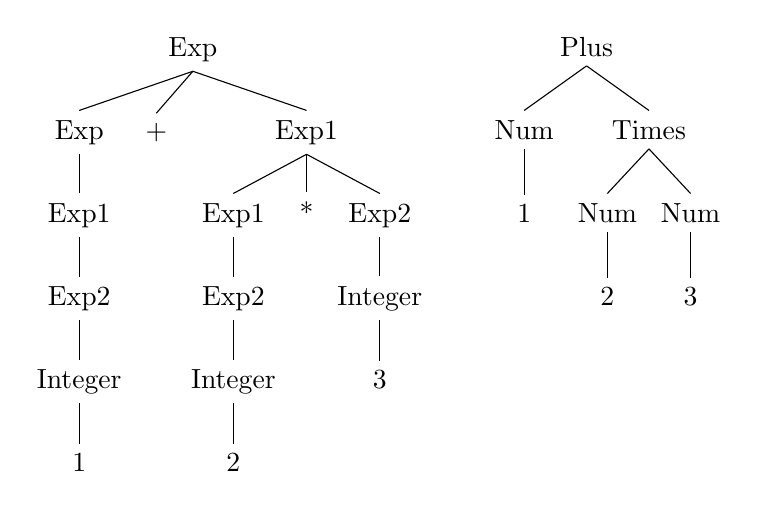
\begin{tikzpicture}
\begin{scope}
\Tree[.Exp [.Exp [.Exp1 [.Exp2 [.Integer $1$ ]]]]
           [.+ ]
           [.Exp1 [.Exp1 [.Exp2 [.Integer $2$ ]]]
                  [.* ]
                  [.Exp2 [.Integer $3$ ]]]]
\end{scope}

\begin{scope}[xshift=5cm]
\Tree[.Plus [.Num $1$ ]
            [.Times [.Num $2$ ]
                    [.Num $3$ ]]]
\end{scope}
\end{tikzpicture}
\hfil

\newpage
The expression $1+(2*3)$:

\hfil
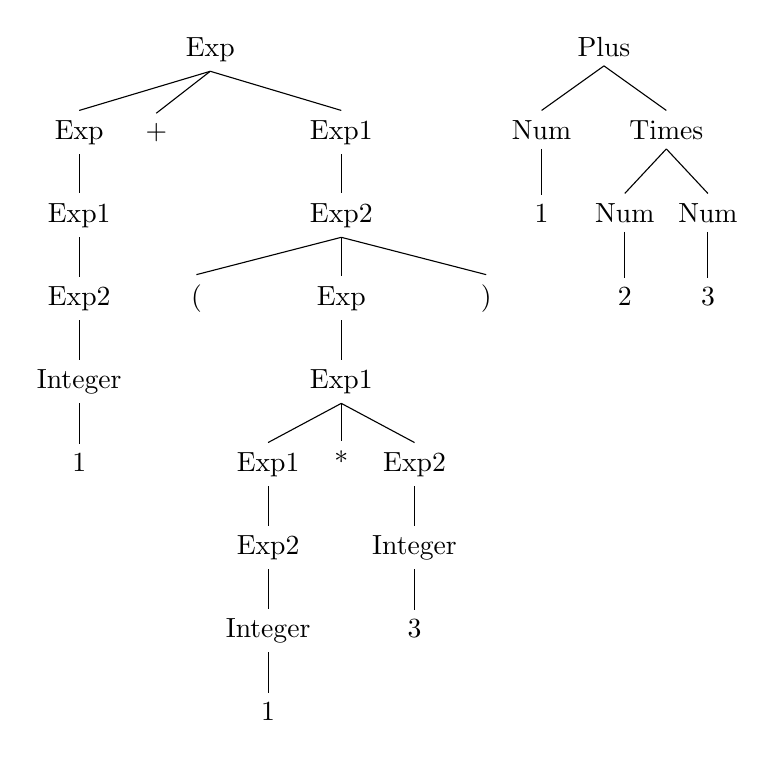
\begin{tikzpicture}
\begin{scope}
\Tree[.Exp [.Exp [.Exp1 [.Exp2 [.Integer $1$ ]]]]
           [.+ ]
           [.Exp1 [.Exp2 [.( ]
                         [.Exp [.Exp1 [.Exp1 [.Exp2 [.Integer $1$ ]]]
                                      [.* ]
                                      [.Exp2 [.Integer $3$ ]]]]
                         [.) ]]]]
                         
\end{scope}

\begin{scope}[xshift=5cm]
\Tree[.Plus [.Num $1$ ]
            [.Times [.Num $2$ ]
                    [.Num $3$ ]]]
\end{scope}
\end{tikzpicture}
\hfil    

The expression $(1+2)*3$:

\hfil
\begin{tikzpicture}
\begin{scope}
\Tree[.Exp [.Exp1 [.Exp1 [.Exp2 [.( ]
                                [.Exp [.Exp [.Exp1 [.Exp2 [.Integer $1$ ]]]]
                                      [.+ ]
                                      [.Exp1 [.Exp2 [.Integer $2$ ]]]]
                                [.) ]]]
           [.* ]
           [.Exp2 [.Integer $3$ ]]]]
                         
\end{scope}

\begin{scope}[xshift=5cm]
\Tree[.Times [.Plus [.Num $1$ ]
                    [.Num $2$ ]]
             [.Num $3$ ]]
\end{scope}
\end{tikzpicture}
\hfil

\newpage
The expression $1+2*3+4*5+6$:

\hfil
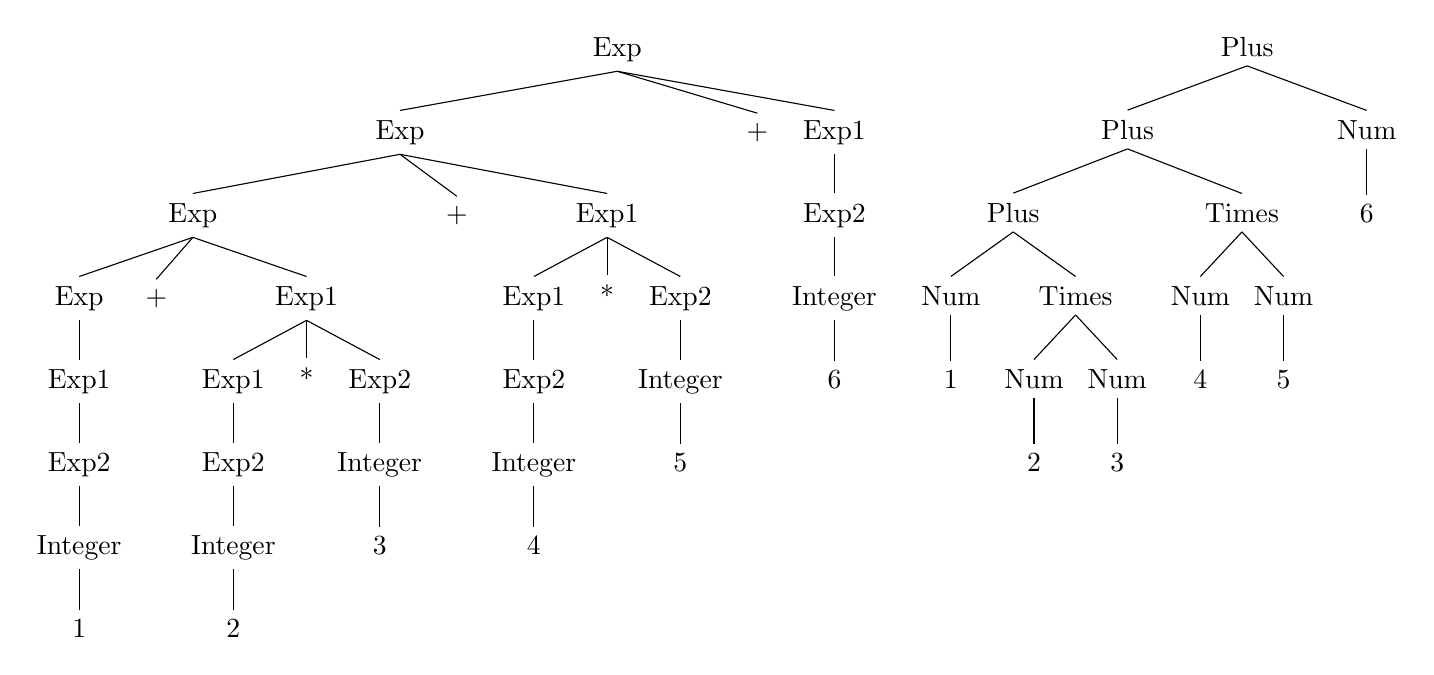
\begin{tikzpicture}
\begin{scope}
\Tree[.Exp [.Exp [.Exp [.Exp [.Exp1 [.Exp2 [.Integer $1$ ]]]]
                       [.+ ]
                       [.Exp1 [.Exp1 [.Exp2 [.Integer $2$ ]]]
                              [.* ]
                              [.Exp2 [.Integer $3$ ]]]]
                 [.+ ]
                 [.Exp1 [.Exp1 [.Exp2 [.Integer $4$ ]]]
                        [.* ]
                        [.Exp2 [.Integer $5$ ]]]]
           [.+ ]
           [.Exp1 [.Exp2 [.Integer $6$ ]]]]
                

                         
\end{scope}

\begin{scope}[xshift=8cm]
\Tree[.Plus [.Plus [.Plus [.Num $1$ ]
                          [.Times [.Num $2$ ]
                                  [.Num $3$ ]]]
                   [.Times [.Num $4$ ]
                           [.Num $5$ ]]]
            [.Num $6$ ]]

                   
\end{scope}
\end{tikzpicture}
\hfil

\noindent \textbf{Analysis of the abstract syntax tree of $1+2+3$}:
The abstract syntax tree of $1+2+3$ would match the tree of $(1+2)+3$. This is because the first breakdown of $+$ separates it to \texttt{Exp} and \texttt{Exp1}, and \texttt{Exp1} cannot reduce down to another sum. Therefore, the right side of the tree must become an integer, while the left side reduces down to a sum. The resulting tree would be as follows, which matches $(1+2)+3$ and not $1+(2+3)$.

\hfil
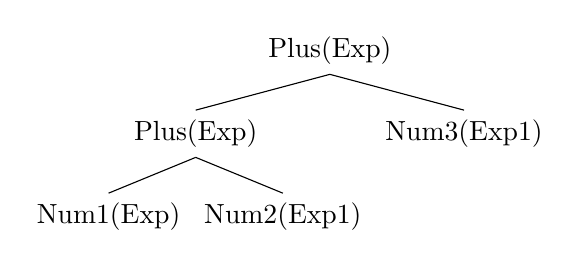
\begin{tikzpicture}
\Tree[.Plus(Exp) [.Plus(Exp) [.Num1(Exp) ]
                             [.Num2(Exp1) ]]
                 [.Num3(Exp1) ]]
\end{tikzpicture}
\hfil

\newpage

\subsection{Week 5}
After generating a working parser demonstrating lambda calculus, linearized abstract syntax trees and 2-dimensional notation abstract syntax trees can be generated for the below expressions.
\begin{lstlisting}[language=Haskell]
-- x
x 
Prog (EVar (Id "x"))
\end{lstlisting}

\hfil
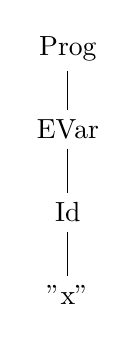
\begin{tikzpicture}
\Tree[.Prog [.EVar [.Id [."x" ]]]]
\end{tikzpicture}
\hfil

\begin{lstlisting}[language=Haskell]
-- x x
x x
Prog (EApp (EVar (Id "x")) (EVar (Id "x")))
\end{lstlisting}

\hfil
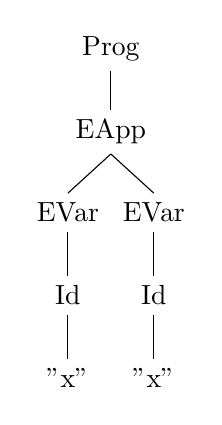
\begin{tikzpicture}
\Tree[.Prog [.EApp [.EVar [.Id [."x" ]]]
                   [.EVar [.Id [."x" ]]]]]
\end{tikzpicture}
\hfil

\begin{lstlisting}[language=Haskell]
-- x y
x y
Prog (EApp (EVar (Id "x")) (EVar (Id "y")))
\end{lstlisting}

\hfil
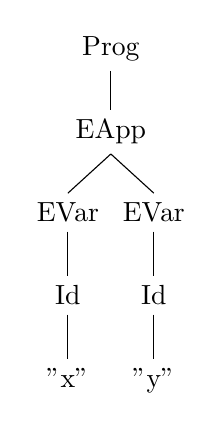
\begin{tikzpicture}
\Tree[.Prog [.EApp [.EVar [.Id [."x" ]]]
                   [.EVar [.Id [."y" ]]]]]
\end{tikzpicture}
\hfil

\begin{lstlisting}[language=Haskell]
-- x y z
x y z
Prog (EApp (EApp (EVar (Id "x")) (EVar (Id "y"))) (EVar (Id "z")))
\end{lstlisting}

\hfil
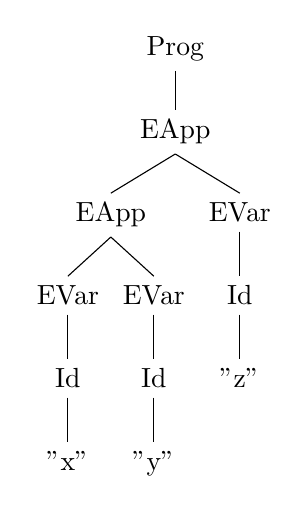
\begin{tikzpicture}
\Tree[.Prog [.EApp [.EApp [.EVar [.Id [."x" ]]]
                          [.EVar [.Id [."y" ]]]]
                   [.EVar [.Id [."z" ]]]]]
\end{tikzpicture}
\hfil

\begin{lstlisting}[language=Haskell]
-- \ x.x
\ x . x
Prog (EAbs (Id "x") (EVar (Id "x")))
\end{lstlisting}

\hfil
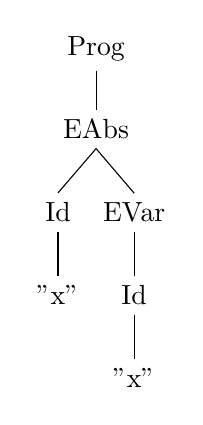
\begin{tikzpicture}
\Tree[.Prog [.EAbs [.Id [."x" ]]
                   [.EVar [.Id [."x" ]]]]]
\end{tikzpicture}
\hfil
\newpage
\begin{lstlisting}[language=Haskell]
-- \ x.x x
\ x . x x
Prog (EAbs (Id "x") (EApp (EVar (Id "x")) (EVar (Id "x"))))
\end{lstlisting}

\hfil
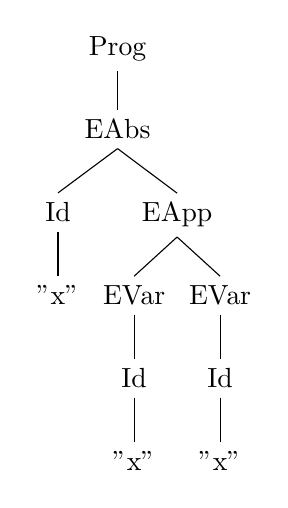
\begin{tikzpicture}
\Tree[.Prog [.EAbs [.Id [."x" ]]
                   [.EApp [.EVar [.Id [."x" ]]]
                          [.EVar [.Id [."x" ]]]]]]
\end{tikzpicture}
\hfil

\begin{lstlisting}[language=Haskell]
-- (\ x . (\ y . x y)) (\ x.x) z
\ x . \ y . x y (\ x . x)z
Prog (EApp (EApp (EAbs (Id "x") (EAbs (Id "y") (EApp (EVar (Id "x")) (EVar (Id "y"))))) (EAbs (Id "x") (EVar (Id "x")))) (EVar (Id "z")))
\end{lstlisting}

\hfil
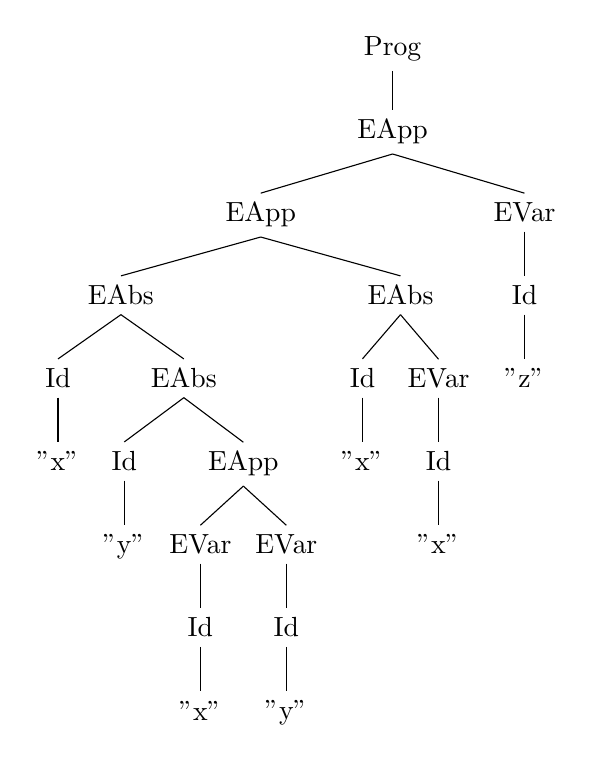
\begin{tikzpicture}
\Tree[.Prog [.EApp [.EApp [.EAbs [.Id [."x" ]]
                                 [.EAbs [.Id [."y" ]]
                                        [.EApp [.EVar [.Id [."x" ]]]
                                               [.EVar [.Id [."y" ]]]]]]
                          [.EAbs [.Id [."x" ]]
                                 [.EVar [.Id [."x" ]]]]]
                   [.EVar [.Id [."z" ]]]]]
\end{tikzpicture}
\hfil

\newpage
\begin{lstlisting}[language=Haskell]
-- (\ x . \ y . x y z) a b c
\ x . \ y . x y z a b c
Prog (EApp (EApp (EApp (EAbs (Id "x") (EAbs (Id "y") (EApp (EApp (EVar (Id "x")) (EVar (Id "y"))) (EVar (Id "z"))))) (EVar (Id "a"))) (EVar (Id "b"))) (EVar (Id "c")))
\end{lstlisting}

\hfil
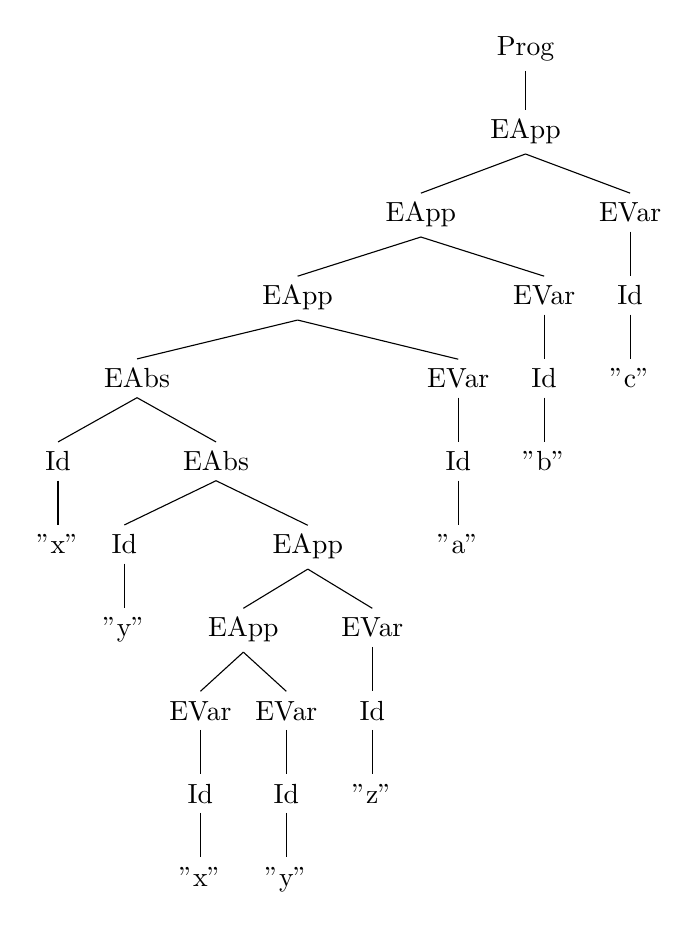
\begin{tikzpicture}
\Tree[.Prog [.EApp [.EApp [.EApp [.EAbs [.Id [."x" ]]
                                        [.EAbs [.Id [."y" ]]
                                               [.EApp [.EApp [.EVar [.Id [."x" ]]]
                                                             [.EVar [.Id [."y" ]]]]
                                                      [.EVar [.Id [."z" ]]]]]]
                                 [.EVar [.Id [."a" ]]]]
                          [.EVar [.Id [."b" ]]]]
                   [.EVar [.Id [."c" ]]]]]
\end{tikzpicture}
\hfil

\noindent The following will show the reduction of several lambda calculus expressions, with the last reduction using the \texttt{evalCBN} method from provided interpreter code.
\begin{lstlisting}[language=Haskell]
(\x.x) a
    = a
\end{lstlisting}
\begin{lstlisting}[language=Haskell]
\x.x a
    = \x.x a
\end{lstlisting}
\begin{lstlisting}[language=Haskell]
(\x.\y.x) a b
    = (\y.a) b
    = a
\end{lstlisting}
\begin{lstlisting}[language=Haskell]
(\x.\y.y) a b
    = (\y.y) b
    = b
\end{lstlisting}
\newpage
\begin{lstlisting}[language=Haskell]
(\x.\y.x) a b c
    = (\y.a) b c
    = a c
\end{lstlisting}
\begin{lstlisting}[language=Haskell]
(\x.\y.y) a b c
    = (\y.a) b c
    = b c
\end{lstlisting}
\begin{lstlisting}[language=Haskell]
(\x.\y.x) a (b c)
    = (\y.a) (b c)
    = a
\end{lstlisting}
\begin{lstlisting}[language=Haskell]
(\x.\y.y) a (b c)
    = (\y.y) (b c)
    = b c
\end{lstlisting}
\begin{lstlisting}[language=Haskell]
(\x.\y.x) (a b) c
    = (\y.(a b)) c
    = a b
\end{lstlisting}
\begin{lstlisting}[language=Haskell]
(\x.\y.y) (a b) c
    = (\y.y) c
    = c
\end{lstlisting}
\begin{lstlisting}[language=Haskell]
(\x.\y.x) (a b c)
    = \y.(a b c)
\end{lstlisting}
\begin{lstlisting}[language=Haskell]
(\x.\y.y) (a b c)
    = \y.y
\end{lstlisting}
\begin{lstlisting}[language=Haskell]
evalCBN (\x.x)((\y.y)a)
    = evalCBN (EApp (EAbs (Id "x") (EVar (Id "x"))) (EApp (EAbs (Id "y") (EVar (Id "y"))) (EVar (Id "a")))) -- converted to concrete format
    = evalCBN (subst (Id "x") (EApp (EAbs (Id "y") (EVar (Id "y"))) (EVar (Id "a"))) (EVar (Id "x"))) -- provided interpreter line 27
    = evalCBN (EApp (EAbs (Id "y") (EVar (Id "y"))) (EVar (Id "a"))) = -- reduction of subst in one step
    = evalCBN (subst (Id "y") (EVar (Id "a")) (EVar (Id "y"))) -- provided interpreter line 27
    = evalCBN (EVar (Id "a")) -- reduction of subst in one step
    = a -- line 32
\end{lstlisting}
\newpage

\subsection{Week 6}
The following is an evaluation of a longer lambda calculus expression.

\begin{lstlisting}[language=Haskell]
-- (\exp . \two . \three . exp two three)
-- (\m.\n. m n)
-- (\f.\x. f (f x))
-- (\f.\x. f (f (f x)))

    = ((\m.\n. m n) (\f.\x. f (f x)) (\f.\x. f (f (f x))))
    = ((\m.\n. m n) (\f.\x. f (f x)) (\f2.\x2. f2 (f2 (f2 x2))))
    = ((\n. (\f.\x. f (f x)) n) (\f2.\x2. f2 (f2 (f2 x2))))
    = ((\f.\x. f (f x)) (\f2.\x2. f2 (f2 (f2 x2))))
    = (\x. (\f2.\x2. f2 (f2 (f2 x2))) ((\f2.\x2. f2 (f2 (f2 x2))) x))
    = (\x. (\x2. ((\f2.\x2. f2 (f2 (f2 x2))) x) (((\f2.\x2. f2 (f2 (f2 x2))) x) (((\f2.\x2. f2 (f2 (f2 x2))) x) x2))))
    = (\x. (\x2. (x (x (x (((\f2.\x2. f2 (f2 (f2 x2))) x) (((\f2.\x2. f2 (f2 (f2 x2))) x) x2)))))))
    = (\x. (\x2. (x (x (x (((\x2. x (x (x x2)))) (((\f2.\x2. f2 (f2 (f2 x2))) x) x2)))))))
    = (\x. (\x2. (x (x (x ((\x2. x (x (x x2))) (((\f2.\x2. f2 (f2 (f2 x2))) x) x2)))))))
    = (\x. (\x2. (x (x (x (x (x (x (((\f2.\x2. f2 (f2 (f2 x2))) x) x2)))))))))
    = (\x. (\x2. (x (x (x (x (x (x ((\x2. x (x (x x2))) x2)))))))))
    = \x. \x2. x (x (x (x (x (x (x (x (x x2))))))))
\end{lstlisting}

\newpage

\subsection{Week 7}
This section will investigate bound and free variables in a lambda-calculus interpreter.

\noindent The following is a section of the interpreter code.
\begin{lstlisting}[language=Haskell]
evalCBN (EApp e1 e2) = case (evalCBN e1) of -- line 5
    (EAbs i e3) -> evalCBN (subst i e2 e3)       -- line 6
    e3 -> EApp e3 e2                             -- line 7
evalCBN x = x                                    -- line 8
\end{lstlisting}

\noindent In this code, all variables (\texttt{e1}, \texttt{e2}, \texttt{e3}, \texttt{i}, and \texttt{x}) are \textbf{bound variables}. This is because the variable names can be changed without changing the function \texttt{evalCBN}.

\noindent \texttt{e1}:\\
Binder: \texttt{evalCBN (EApp e1 e2)}\\
Scope: \texttt{case (evalCBN e1) of
| (EAbs i e3) -> evalCBN (subst i e2 e3)
| e3 -> EApp e3 e2}

\noindent \texttt{e2}:\\
Binder: \texttt{evalCBN (EApp e1 e2)}\\
Scope: \texttt{case (evalCBN e1) of
| (EAbs i e3) -> evalCBN (subst i e2 e3)
| e3 -> EApp e3 e2}

\noindent \texttt{e3}:\\
Binder (line 6): \texttt{EAbs i e3}\\
Scope (line 6): \texttt{evalCBN (subst i e2 e3)}\\
Binder (line 7): \texttt{e3}\\
Scope (line 7): \texttt{EApp e3 e2}

\noindent \texttt{i}:\\
Binder: \texttt{EAbs i e3}\\
Scope: \texttt{evalCBN (subst i e2 e3)}

\noindent \texttt{x}:\\
Binder: \texttt{evalCBN x}\\
Scope: \texttt{x}

\newpage

The following is another section of the interpreter code.
\begin{lstlisting}[language=Haskell]
subst id s (EAbs id1 e1) =           -- line 18
let f = fresh (EAbs id1 e1)          -- line 20
    e2 = subst id1 (EVar f) e1 in   -- line 21
    EAbs f (subst id s e2)           -- line 22
\end{lstlisting}

\noindent In this code, all variables (\texttt{id}, \texttt{s}, \texttt{id1}, \texttt{e1}, \texttt{f}, and \texttt{e2}) are \textbf{bound variables}. This is because the variable names can be changed without changing the function \texttt{subst}.

\noindent \texttt{id}:\\
Binder: \texttt{subst id s (EAbs id1 e1)}\\
Scope: \texttt{let f = fresh (EAbs id1 e1) | e2 = subst id1 (EVar f) e1 in | EAbs f (subst id s e2)}

\noindent \texttt{s}:\\
Binder: \texttt{subst id s (EAbs id1 e1)}\\
Scope: \texttt{let f = fresh (EAbs id1 e1) | e2 = subst id1 (EVar f) e1 in | EAbs f (subst id s e2)}

\noindent \texttt{id1}:\\
Binder: \texttt{subst id s (EAbs id1 e1)}\\
Scope: \texttt{let f = fresh (EAbs id1 e1) | e2 = subst id1 (EVar f) e1 in | EAbs f (subst id s e2)}

\noindent \texttt{e1}:\\
Binder: \texttt{subst id s (EAbs id1 e1)}\\
Scope: \texttt{let f = fresh (EAbs id1 e1) | e2 = subst id1 (EVar f) e1 in | EAbs f (subst id s e2)}

\noindent \texttt{f}:\\
Binder: \texttt{let f}\\
Scope: \texttt{fresh (EAbs id1 e1) | e2 = subst id1 (EVar f) e1 in | EAbs f (subst id s e2)}

\noindent \texttt{e2}:\\
Binder: \texttt{e2}\\
Scope: \texttt{subst id1 (EVar f) e1 in | EAbs f (subst id s e2)}

\noindent\rule{\textwidth}{1pt}

\noindent Another example of \texttt{evalCBN} from a provided interpreter snippet is demonstrated here, now including the above snippet for \texttt{fresh}:

\begin{lstlisting}[language=Haskell]
evalCBN (\x.\y.x) y z =
    = evalCBN (EApp (EApp (EAbs (Id "x") (EAbs (Id "y") (EVar (Id "x")))) (EVar (Id "y"))) (EVar (Id "z"))) -- converted to concrete format
    = evalCBN (EApp (evalCBN (EApp (EAbs (Id "x") (EAbs (Id "y") (EVar (Id "x")))) (EVar (Id "y")))) (EVar (Id "z"))) -- line 5
    = evalCBN (EApp (evalCBN (subst (Id "x") (EVar (Id "y")) (EAbs (Id "y") (EVar (Id "x"))))) (EVar (Id "z"))) -- line 6
    = evalCBN (EApp (evalCBN (EAbs (Id "y0") (subst (Id "x") (EVar (Id "y")) (subst (Id "y") (EVar (Id "y0")) (EVar (Id "x")))))) (EVar (Id "z"))) -- line 22
    = evalCBN (EApp (evalCBN (EAbs (Id "y0") (subst (Id "x") (EVar (Id "y")) (EVar (Id "x"))))) (EVar (Id "z"))) -- line 16
    = evalCBN (EApp (evalCBN (EAbs (Id "y0") (EVar (Id "y")))) (EVar (Id "z"))) -- line 15
    = evalCBN (EApp (EAbs (Id "y0") (EVar (Id "y"))) (EVar (Id "z"))) -- line 8
    = evalCBN (subst (Id "y0") (EVar (Id "z")) (EVar (Id "y"))) -- line 6
    = evalCBN (EVar (Id "y")) -- line 16
    = y -- line 8
\end{lstlisting}

\newpage 

The following is an analysis of several abstract reduction systems.

\noindent \texttt{A=\{\}}\\
A picture will not be drawn for this, for it is just an empty set. This ARS is terminating because an empty set cannot reduce any further. It is confluent because there is no divergence of elements. It has unique normal forms (which is the empty set).

\noindent\rule{\textwidth}{1pt}

\noindent \texttt{A=\{a\} and R=\{\}}\\
A picture will not be drawn for this, for it is just \texttt{a}. This ARS is terminating because \texttt{a} cannot reduce any further. It is confluent because there is no divergence of elements. It has unique normal forms (which is \texttt{a}).

\noindent\rule{\textwidth}{1pt}

\noindent \texttt{A=\{a\} and R=\{(a,a)\}}
\begin{center}
    \includegraphics[scale=0.5]{ars3.png}
\end{center}
This ARS is not terminating because \texttt{a} can always reduce to itself. It is confluent because the divergence of \texttt{a} can converge back to itself. It does not have unique normal forms, as \texttt{a} can always reduce to itself.

\noindent\rule{\textwidth}{1pt}

\noindent \texttt{A=\{a,b,c\} and R=\{(a,b),(a,c)\}}
\begin{center}
    \includegraphics[scale=0.5]{ars4.png}
\end{center}
This ARS is terminating because it cannot reduce any further than \texttt{b} or \texttt{c}. It is not confluent since the divergence to \texttt{b} and \texttt{c} cannot converge back. It does not have unique normal forms, as there are two normal forms of \texttt{a} (\texttt{b} and \texttt{c}).

\noindent\rule{\textwidth}{1pt}

\noindent \texttt{A=\{a,b\} and R=\{(a,a),(a,b)\}}
\begin{center}
    \includegraphics[scale=0.5]{ars5.png}
\end{center}
This ARS is not terminating because \texttt{a} can always reduce further. It is confluent because the divergence to \texttt{a} and \texttt{b} can converge back, with the recursive \texttt{a} converging back to the original \texttt{b}. It has unique normal forms, as \texttt{a} has the unique normal form of \texttt{b}.

\newpage

\noindent \texttt{A=\{a,b,c\} and R=\{(a,b),(b,b),(a,c)\}}
\begin{center}
    \includegraphics[scale=0.5]{ars6.png}
\end{center}
This ARS is not terminating because \texttt{b} can always reduce further. It is not confluent since the divergence to \texttt{b} and \texttt{c} cannot converge back. It does not have unique normal forms, as there are two normal forms of \texttt{a} (\texttt{b} and \texttt{c}).

\noindent\rule{\textwidth}{1pt}

\noindent \texttt{A=\{a,b,c\} and R=\{(a,b),(b,b),(a,c),(c,c)\}}
\begin{center}
    \includegraphics[scale=0.5]{ars7.png}
\end{center}
This ARS is not terminating because \texttt{b} and \texttt{c} can always reduce further. It is not confluent since the divergence to \texttt{b} and \texttt{c} cannot converge back. It does not have unique normal forms, as there are two normal forms of \texttt{a} (\texttt{b} and \texttt{c}).
\newpage
Lastly, the 8 different cases of confluence, termination, and presence of unique normal forms are shown below.

\begin{center}
\begin{tabular}{ | m{5em} | m{5em}| m{12em} | m{3.2cm} | }
 \hline
 Confluent & Terminating & Has unique normal forms & Example \\
 \hline\hline
 True & True & True & \includegraphics[scale=0.5]{ex1.png} \\ 
 \hline
 True & True & False & If an ARS is confluent and terminating then all elements reduce to a unique normal form. \\
 \hline
 True & False & True & \includegraphics[scale=0.5]{ex3.png} \\
 \hline
 True & False & False & \includegraphics[scale=0.5]{ex4.png} \\
 \hline
 False & True & True & An ARS has unique normal forms if (and only if) it is confluent and normalising. \\
 \hline
 False & True & False & \includegraphics[scale=0.5]{ex6.png} \\
 \hline
 False & False & True & An ARS has unique normal forms if (and only if) it is confluent and normalising. \\
 \hline
 False & False & False & \includegraphics[scale=0.5]{ex8.png} \\
 \hline
\end{tabular}
\end{center}

\newpage

\subsection{Week 8}
The following will investigate properties of the following rewrite system:
\begin{lstlisting}
aa -> a
bb -> b
ba -> ab
ab -> ba
\end{lstlisting}

\noindent \textbf{Why does the ARS not terminate?: } This ARS does not terminate because of the final two rules. There is a cycle between the strings \texttt{ab} and \texttt{ba}, meaning that there is no end to the cycle if there exists either of these strings.\\

\noindent \textbf{What are the normal forms?: } The normal forms of this ARS are therefore an empty string, \texttt{a}, and \texttt{b}. Any string longer than one character with just \texttt{ab} and \texttt{ba} will be rewritten as another same-length string, as per the rewrite rules.\\

\noindent \textbf{Modify the ARS so that it is terminating, has unique normal forms: } These rewrite rules can be slightly altered so that the ARS is terminating and has unique normal forms. By removing the fourth rule, it eliminates the possibility of the original termination problem. What this does is allow a combination of \texttt{a} and \texttt{b} through only one permutation. This would end up adding another normal form to the previously mentioned three, which is \texttt{ab}.

This works because the functionality of the ARS is preserved. Going through the 4 possible combinations of two-letter strings, \texttt{aa} and \texttt{bb} reduce in the same fashion. In order to prevent termination, the third or fourth rule should be eliminated. The fourth rule was chosen to be eliminated here to keep the alphabetical orderliness of \texttt{ab}. Therefore, the third rule reduces the same and the elimination of the fourth rule causes \texttt{ab} to be a normal form.\\

\noindent \textbf{Describe the specification implemented by the ARS: } The specification can be found by seeing the patterns that emerge from reduction using this ARS. This can be done by coming up with possible invariants. Looking at the rules, it can be guessed that any string with the normal form \texttt{a} or \texttt{b} only contained the letter \texttt{a}/\texttt{b} in the beginning string, respectively. If a string contained both \texttt{a} and \texttt{b}, the third rewrite rule would be used eventually, leading to the normal form of \texttt{ab}. 

Therefore, an invariant that can be concluded is that \textbf{the original string only contained \texttt{a}'s if the normal form of the string is \texttt{a}}. The same invariant applies to \texttt{b} as well. Likewise, \textbf{the original string contained \texttt{a}'s and \texttt{b}'s if the normal form of the string is \texttt{ab}}. Finally, \textbf{the original string contained neither \texttt{a}'s nor \texttt{b}'s if the normal form of the string is an empty string}. All of these invariants assume that the only possible letters that can appear in the string are \texttt{a} and \texttt{b}.

The specification can then be constructed to describe the ARS as a function that determines the presence of \texttt{a}'s and the presence of \texttt{b}'s at the same time. The 4 possible combinations of \texttt{a}'s and \texttt{b}'s presences can be matched up to the 4 possible normal forms of the ARS.

\newpage

\subsection{Week 9}

This section involves an analysis of the following ARS:
\begin{lstlisting}
ba -> ab            aa -> b
ab -> ba            ab -> c
ac -> ca            ac ->  
ca -> ac            bb ->
bc -> cb            cb -> a
cb -> bc            cc -> b
\end{lstlisting}

\noindent The first thing to note is that with this ARS, the order of the letters do not matter. Any combination of letters can be reoriented within the entire string, hinting that the specification has something to do with commutativity. The second thing to note is that this ARS is terminating with 4 normal forms: \texttt{a}, \texttt{b}, \texttt{c}, and the empty list. This can be shown since the second half of the rules reduce any two-letter string to a one- or zero-letter string, and this cycle would continue until one of the 4 normal forms are reached. 

This can be formalized as an important invariant, which is that every two-letter combination yields a single character. The empty list will be treated as a single character for now, as this is important in the explanation.

Combining these two observations and the invariant, it hints at arithmetic, namely addition and modulo. Using this as a guide, the letters in this ARS can be treated as base-10 numbers instead, with $a=1$, $b=2$, and $c=3$. Pairs of letters together will be interpreted as the addition of those two numbers, with \texttt{aa} acting as $a+a$ as an example. This helps decipher the first half of the ruleset, as it reinforces the fact that adding two letters together can be done in either order (commutativity), and it will yield the same result in the second half of the ruleset.

The 4 normal forms can also be treated as these base-10 numbers, with the empty list acting as $0$. Doing this to the second half of the ruleset, we get the following substitution:

\begin{lstlisting}
1 + 1 -> 2
1 + 2 -> 3
1 + 3 -> 0
2 + 2 -> 0
3 + 2 -> 1
3 + 3 -> 2
\end{lstlisting}

Seeing this substitution, this can be seen to follow the pattern of \texttt{mod 4}. Therefore, the specification for this ARS is that it calculates \texttt{n mod 4}, with \texttt{n} being the sum of a given word's letters, as if they were treated as base-10 numbers. This takes advantage of another hidden invariant, which is the following:

\texttt{(((x+y) mod 4)+z) mod 4 = (x+y+z) mod 4}, $\forall x, y, z \in\mathbb{N}$

To give a longer example, \texttt{abcb} should reduce to the empty list, as $(1+2+3+2)mod4 = 0$. We can see this does indeed work with the following possible reductions.

\begin{lstlisting}
Reduction 1: abcb -> ccb -> bb -> []
Reduction 2: abcb -> ccb -> ca -> ac -> []
Reduction 3: abcb -> acbb -> aab -> bb -> []
Reduction 4: abcb -> acbb -> aab -> ac -> []
Reduction 5: abcb -> aba -> ca -> ac -> []
Reduction 6: abcb -> aba -> aab -> ac -> []
\end{lstlisting}

\newpage

\subsection{Week 10}
The following is a calculation involving a fixed-point combinator and its computation rule. The calculation solves $fix_F 2$ using equational reasoning. 

\begin{lstlisting}[language=Haskell]
fix_F 2 = F fix_F 2                                                -- computation rule of fix_F
         = (\n. if n == 0 then 1 else n * fix_F (n-1)) 2           -- definition of F and beta reduction
         = if 2 == 0 then 1 else 2 * fix_F (2-1)                   -- beta reduction of n
         = 2 * (fix_F 1)                                           -- computation rule of if/then/else
         = 2 * (F fix_F 1)                                         -- computation rule of fix_F
         = 2 * (\n. if n == 0 then 1 else n * fix_F (n-1)) 1       -- definition of F and beta reduction
         = 2 * (if 1 == 0 then 1 else 1 * fix_F (1-1))             -- beta reduction of n
         = 2 * (1 * fix_F 0)                                       -- computation rule of if/then/else
         = 2 * (1 * F fix_F 0)                                     -- computation rule of fix_F
         = 2 * (1 * (\n. if n == 0 then 1 else n * fix_F (n-1)) 0) 
                                                                   -- definition of F and beta reduction
         = 2 * (1 * (if 0 == 0 then 1 else 0 * fix_F (0-1)))       -- beta reduction of n
         = 2 * (1 * (1))                                           -- computation rule of if/then/else
         = 2                                                       -- multiplication
\end{lstlisting}
\newpage

\subsection{Week 11}

The following is an essay comprised of my thoughts and analysis on the world of composing financial contracts through a domain specific programming language.\\


Domain specific programming languages (DSL) are programming languages that are specialized to a specific application or purpose. Common applications today that include the use of DSLs are Microsoft Excel and musical notation software. Certain programming languages also serve as DSLs, such as R (statistics) and HTML (web design). The worlds of programming and finance don’t seem to have much relation at first, but the number of ways where they could be co-beneficial in today’s technology-driven world is only increasing. Encoding financial contracts through a DSL is seen to have many practical applications. Condensing a wide range of possible contracts into something easier to understand, as well as using these contracts to present information effectively, are some notable advantages that a DSL could have in the financial world.

There are many details that go into creating a generic financial contract. Dates, amounts, conditions, and currency are only a select few of details that make up a contract. By encoding these contracts through a DSL, the format of a contract can be standardized within its own special language. After figuring out what key details can be altered to define a contract, the DSL can describe any contract imaginable with a given set of these important details. A set of variables, or “combinators”, would be used to represent these details, but the generic body of a contract would be universal throughout all contracts. This makes it easier for contracts to be conceptualized, with only the key details needing attention.

A key advantage of standardizing these contracts through a programming language is that special operations can be done on these digital contracts. For example, one can combine different contracts if a contract requires two payments at different times. This requires less knowledge and effort than composing a new contract altogether, whether physical or digital. Additionally, one can scale a contract based on another observable combinator. This means that one can define a contract’s value solely based on a scaled version of another variable, meaning the value would automatically be calculated given the other variable. One can also see visual interpretations of these contracts to understand them easier, such as “presenting contracts in new graphical ways” and “providing animated simulations” (Source). This might help others to see the value in a contract easier, as well as help financial experts make important decisions based on the contracts.

Although there are many benefits to digitalizing contracts, it comes with a few questions about its practicality. Security and legality are important aspects of physical contracts today, so its digital counterpart would need to be thought out as well. Human behavior would still be an important factor in creating these contracts, so a safeguard to prevent exploitative practices would be necessary. Neutrality in many aspects should be ensured to keep fairness and visibility in this kind of program. For example, a more experienced programmer should not have some kind of advantage over a lesser experienced programmer. Additionally, a DSL’s usage in other fields could be investigated more to make simplifying other processes easier. Even if learning this specific DSL perfectly had no beneficial effect to using these contracts, it can be beneficial outside of creating contracts. Programming is widely known as an essential skill in many fields, and it can still prove to be useful at least somewhere else, since financial engineering combines two big seemingly-unrelated fields. In all, a DSL can drastically expand the possibilities of one field’s standards, as “a single formal description can drive all manner of automated processes” (Source).\\


Source: 
\href{https://www.cs.tufts.edu/~nr/cs257/archive/simon-peyton-jones/contracts.pdf}{Composing Contracts: An Adventure in Financial Engineering}

\newpage

\subsection{Week 12}

The following is an analysis of the following code through the lens of Hoare logic:

\texttt{while (x!=0) do z:=z*y;  x:= x-1 done}

Looking at the short program, the program will terminate only if $x > 0$ before the while loop begins. The program will also calculate $z = y^x$ if $z = 1$ before the while loop.

To find the invariant for this while loop, a table of execution can be made. The example initialization will be $x = 10$, $y = 2$, and $z = 1$. \texttt{t} will be used to count the number of iterations so far in the while loop.

\begin{center}
\begin{tabular}{ | c | c | c | c| }
    \hline
    \texttt{t} & \texttt{x} & \texttt{y} & \texttt{z} \\
    \hline\hline
    0 & 10 & 2 & 1 \\ 
    \hline
    1 & 9 & 2 & 2 \\
    \hline
    2 & 8 & 2 & 4 \\
    \hline
    ... & ... & ... & ... \\
    \hline
    9 & 1 & 2 & 512 \\
    \hline
    10 & 0 & 2 & 1024 \\
    \hline
\end{tabular}
\end{center}

These numbers satisfy the following invariants:

\begin{itemize}
    \item $t + x = 10$
    \item $z = y ^ t$
\end{itemize}

Using algebra, these two equations can be modified to get an invariant consisting of only \texttt{x}, \texttt{y}, and \texttt{z}: $z = y^{(10 - x)}$.

This can be formalized through a Hoare triple:

\texttt{\{$z = y^{(n - x)}$\}  while (x != 0) do z:=z*y;  x:= x-1 done  \{$z = y^{(n - x)}$\}}

This can be proved from the intended purpose of this for loop with the following starting Hoare triple:

\texttt{\{$z=1 \land x=n$\}  while (x != 0) do z:=z*y;  x:= x-1 done  \{$z = y^n$\}}

To prove this, it must be shown that the precondition implies the invariant and that the invariant implies the postcondition.

To show that the precondition implies the invariant, it must be shown that $z=1 \land x=n$ implies $z = y^{(n - x)}$. If $z=1$ and $x=n$, the second equation reduces to $1=y^0$, or $1=1$. This is always true.

To show that the invariant implies the postcondition, it must be shown that $z = y^{(n - x)}$ implies $z = y^n$. This is true because of the end assumption that $x=0$ when the while loop terminates. Therefore, the first equation reduces to $z = y^n$, making both equations the same and thus the implication true.

\newpage

\section{Project}\label{project}

This section will contain all details for my final software project of this course.

\subsection{Specification}

For my final project, I plan to learn a new programming language, give a concise but informative tutorial on it, and develop a software project that ties in to the course material. 

For this project, I plan to learn the programming language Ruby. Learning a new popular language could be beneficial for personal purposes. My goal is to both learn a relevant language and utilize some concepts learned in the course to create a meaningful project that represents my knowledge of programming languages. With this tutorial, I will create a concise overview of certain topics in general programming, as well as create exercises with their respective solutions for the reader to attempt. This can help reinforce the knowledge gained from the tutorial, and could motivate the reader to look more into the capabilities of Ruby.

As for the software project portion, the goal will be to utilize knowledge gained from the tutorial to understand what it takes to build a web application using Ruby on Rails. Also known as simply "Rails", it is a full-stack web framework that aids in creating powerful web applications. It is a big reason that the Ruby language has gained traction in the first place, so building a software project with this framework would help understand the Ruby language and its real-world applications at a deeper level. The software project in question will be a simple version of a web blog application. The walkthrough will go over the fundamentals of building a barebones Rails application, as well as how one could implement key features of a typical Rails project.

\subsection{Prototype}
Regarding the final project, the following deadlines will be made to keep track of progress of my programming language exploration. Below each deadline are the corresponding finished portions of the software project.\\

\noindent \textbf{November 13, 2022}: Create a tutorial that covers the evolution of Ruby and the fundamentals of the programming language. The tutorial part will cover these categories: basics, control structures, and collections. Exercises and their answers will be provided.
\begin{itemize}
    \item \href{https://hackmd.io/@evrahnos/HJZPgUjSi}{The Ruby tutorial}
    \item \href{https://hackmd.io/@evrahnos/SkWAtPoBs}{Ruby tutorial exercises}
    \item \href{https://hackmd.io/@evrahnos/S1oUsvoBs}{Ruby tutorial solutions}
\end{itemize}

\noindent \textbf{November 20, 2022}: The software project portion will cover an example blog application using the Ruby on Rails framework, going over key aspects of what it takes to create such an application with Rails (for example, show snippets of code demonstrating different functionalities). This milestone will check if a completed first draft is made, which will contain just a walkthrough section.
\begin{itemize}
    \item The walkthrough section of \href{https://hackmd.io/@evrahnos/ryTuitp8o}{Creating a blog with Ruby on Rails}
\end{itemize}

\noindent \textbf{November 27, 2022}: Have the software project complete within the tutorial. As per the previous milestone, the project will cover an example blog application using the Ruby on Rails framework. For this milestone, it will include a final version of the walkthrough, as well as final takeaways after the completion of this project.
\begin{itemize}
    \item The entirety of \href{https://hackmd.io/@evrahnos/ryTuitp8o}{Creating a blog with Ruby on Rails}
\end{itemize}

\newpage

\subsection{Documentation}

The entire tutorial's documentation can be found at the following HackMD link:

\href{https://hackmd.io/@evrahnos/rJyCCKdri}{The Ruby Tutorial}

\subsection{Critical Appraisal}

This software project built on top of the knowledge gained from learning Ruby, with most of knowledge being showcased through the tutorial and exercises. However, the web development aspect contained a little bit of review for me. Having experience with other web development projects, I was familiar with the general flow and structure of creating a website. Comparing Rails to my previous experience with Python's Flask web framework, I noticed some advantages and disadvantages to both. Writing the walkthrough to the blog project in Rails made me better understand why Rails is seen as a powerful development tool.

Throughout this software project, I learned that development preferences can heavily shape opinions on what web framework is best to use. Coming from an extensive Python background, I found the Flask framework to be easy to use when first learning it. With only a recent deep dive into Ruby, I was still getting used to Rails syntax and structure. Nonetheless, coming from a different framework showed me pros and cons to using Flask and Rails. When it comes to simplicity, I would prefer to use Flask. Its syntax is on average much cleaner than Rails, and it is mainly intuitive. Not many extra files need sorting through, and website routes are easily created through just an \texttt{html} file and a route method. When it comes to organization, I would prefer Rails over Flask. Although there are more things to keep track of in Ruby, it is more explicit in nature and has more of an orderly structure to it. For example, Rails's concept of controllers is not really used in Flask. Controllers outline the interactions between viewable data and data manipulation, and defining these can be really helpful when reading the code, such as collaborating on a Rails project within a project group.

This ties in with the main challenge I had undertaking this project, which was learning the different kinds of files and paths Rails uses to create a project. As the concept of controllers are not as present in Flask, it was initially hard to see why it was important to include them. This was a similar case for various other topics in Rails project, such as models and views. Once everything clicked together, I started to understand Rails's special structure and gradually became more used to its syntax. I believe part of this has to do with the fact that Rails documentation is rather sparse, and so clear answers to questions I had about its structure were not easily found.

An interesting observation I made is that my experience with Rails closely matches the common conception of development being faster than other frameworks. Syntax was more complicated than Flask in my opinion, but development time was definitely way shorter than the amount of time it would take for me to develop the same project in Flask.
Even though Rails definitely had a steeper learning curve, learning it definitely pays off for its intended purpose of quick start-up development.

Overall, Rails did a great job balancing user friendliness and performance, as Ruby's goal of user happiness was shown through explicitness and wide use of conventions. This entire project made me think about the concept of structure versus speed in the context of programming languages as a whole. It made me wonder how much performance and development speed would be affected if grammar of the course's imperative programming language interpreter was altered. I would imagine a perfect balance between adaptability and performance would characterize an experienced programmer's ideal language.

\newpage

\section{Conclusions}\label{conclusions}

This course covered building modern functional programming languages from the ground up, starting as small as syntax trees and ending with complex functions using a specified grammar. Starting at the beginning, pattern matching proved to be a very powerful and useful tool when considering the function of a language. The earlier homeworks heavily emphasized this importance, and it helped me understand on a broader level how pattern matching can define how a programming language functions. It made me realize that I use pattern matching unknowingly in everyday life, and this was shown to me through pattern matching exercises involving arithmetic. This was helpful for the transition into syntax trees and lambda calculus, where the true base for these programming languages was shown. 

In all, I have truly learned a lot behind the logic of creating something like this. Stepping back from the specifics of the course, it showed me how versatile programming can be, even in its bare roots. Modern programming languages today often highlight a core purpose, with Ruby emphasizing user friendliness as an example. Creators of programming languages can choose freely how they want their language to be used, whether it be through grammar or language structure. Simple things such as syntax decisions can define how a program runs and looks. That is why the most important takeaway of this course to me is how powerful of a tool versatility is. 

This ties into a big part of the significance of learning programming language theory to me, which is that it is universal. Knowing how a language is built can help understand things between all languages, like design decisions and a language’s pros and cons. At a deeper level, it teaches what the building blocks of a language are made of themselves. For example, a programmer may know how a certain algorithm works (such as building a linked list), but knowing how that algorithm operates within the confines of that specific language can help the programmer understand what they are coding on a deeper level. This leads to some positive effects such as easier debugging and cleaner code.

In other words, knowing the theory behind the programming language I am coding in makes me both more knowledgeable and more skilled as a problem solver. I can now understand why the language functions as it does, and why coding something may be beneficial if done one way over the other. The course has taught me to think of myself not just as a programmer, but as a problem solver that knows the intricacies of what they are programming.

\end{document}